\documentclass[11pt]{latex/exercise}

\input{latex/opts_mths24} 
\setlecturers{Eugeny Epelbaum / Adam Szczepaniak}
\settutors{XXX, YYY}
\setsheetnumber{4}
\setexdate{Thursday, 18 July 2024}

\begin{document}
\makeheader

\morning

\material{
\item Intro to EFT (general idea, integrating out heavy particles, renormalization in QFT, power counting, the principles of an EFT)
\item Intro to ChPT (chiral symmetry of QCD, effective Lagrangian for pions, generalization to the nucleon sector, HB expansion)
\item Beyond perturbation theory: Pionless EFT for two nucleons (renormalization conditions and power counting schemes)
\item Intro to chiral EFT for few-nucleon systems (low-energy theorems and the MERE, KSW approach for perturbative pions, nonperturbative inclusion of pions, renormalization, methods to derive nuclear forces)
}{
\item Feynman diagrams and formulary of QFT:
K. Kumeric, Feynman Diagrams for Beginners, arXiv:1602.04182 [physics.ed-ph]

\item EFTs:
\begin{itemize}
    \item Antonio Pich, Effective Field Theory, hep-ph/9806303
    \item Ira Rotstein, TASI lectures on effective field theories, hep-ph/0308266
    \item David Kaplan, Five lectures on effective field theory, nucl-th/0510023
    \item Aneesh Manohar, Introduction to Effective Field Theories, arXiv:1804.05863 [hep-ph]
    \item Matthias Neubert, Renormalization Theory and EFTs, arXiv:1901.06573 [hep-ph]
\end{itemize}
\item ChPT Reviews:
\begin{itemize}
    \item Bernard, Kaiser, Mei{\ss}ner, Int. J. Mod. Phys. E4 (1995) 193
    \item Pich, Rep. Prog. Phys. 58 (1995) 563
    \item Bernard, Prog. Part. Nucl. Phys. 60 (2007) 82
    \item Scherer, Prog. Part. Nucl. Phys. 64 (2010) 1
\end{itemize}
\item ChPT Lectures:
\begin{itemize}
    \item Scherer, Adv. Nucl. Phys. 27 (2003) 277
    \item Gasser, Lect. Notes Phys.  629 (2004) 1
    \item Text books:
    \item Scherer, Schindler, A Primer for Chiral Perturbation Theory, Springer, Lecture Notes in Physics, 2012
    \item Mei{\ss}ner, Rusetsky, Effective Field Theories
\end{itemize}
\item Chiral EFT for few-N:
Epelbaum, Nuclear forces from chiral effective field theory: A primer, arXiv:1001.3229 [nucl-th]
}

\afternoon

\newcommand{\dd}{\mathrm{d}}
\newcommand{\eins}{\mathds{1}}
\newcommand{\vs}{\slashed{v}}
\renewcommand{\L}{\mathcal{L}}


%%%%%%%%%%%%%%%%%%%%%%%%%%%%%%%%%%%%%%%%%%%%%%%%%%%%%
\definecolor{darkred}{rgb}{0.55, 0.0, 0.0}
\definecolor{debianred}{rgb}{0.84, 0.04, 0.33}

\subsection{Field redefinition}

\noindent
Using the path integral formalism of quantum field theory, one notices that physical observables are independent of field redefinitions
$\phi\rightarrow\phi+f(\phi/\Lambda)$, where $\Lambda$ is a dimensionful parameter. This redefinition does not affect observables, because the integration in the generating functional $Z[J]$ is done over all configurations of $\phi$ and the measure $\mathcal{D}\phi$ compensates any changes of variables due to the Jacobian.  Note that one can drop the additional interpolating field in the part containing the external current $J$ (and work just with $J\phi$) without changing the S-matrix (though Green's functions do change!).

In this exercise we consider the free scalar theory for a field $\phi$ and will demonstrate that the amplitude for $\phi\phi\rightarrow\phi\phi$ scattering is not affected by the field redefinition
\begin{gather}
    \phi\rightarrow \phi+\frac{\phi^2}{\Lambda}.
\end{gather}
\begin{itemize}
    \item[(a)] Transform the Lagrangian for a
          free real scalar field $\phi$ with mass $m$ under the above field redefinition.
    \item[(b)] By applying functional derivatives as summarized in appendix \ref{A:1}, show that the Feynman rules for all of the four interaction parts are given as
          \begin{align}
               & 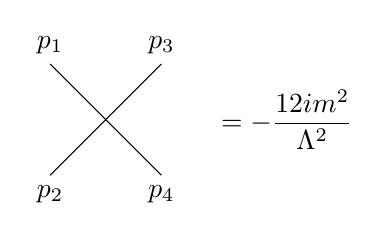
\begin{tikzpicture}
                     \draw (135:1)node[above]{$p_1$}--(0,0)node[midway, rotate=-135]{\myarrow};
                     \draw (225:1)node[below]{$p_2$}--(0,0)node[midway, rotate=-45]{\myarrow};
                     \draw (45:1)node[above]{$p_3$}--(0,0)node[midway, rotate=135]{\myarrow};
                     \draw (-45:1)node[below]{$p_4$}--(0,0)node[midway, rotate=45]{\myarrow};
                     \vertex{0,0}{1};
                     \node at(2.3,0){$\displaystyle=-\frac{12im^2}{\Lambda^2}$};
                 \end{tikzpicture}
              \\
               & 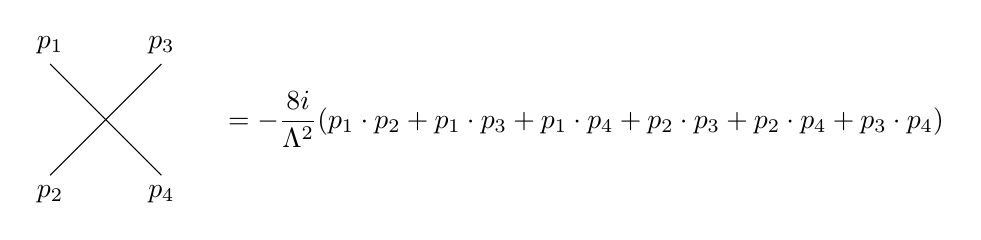
\begin{tikzpicture}
                     \draw (135:1)node[above]{$p_1$}--(0,0)node[midway, rotate=-135]{\myarrow};
                     \draw (225:1)node[below]{$p_2$}--(0,0)node[midway, rotate=-45]{\myarrow};
                     \draw (45:1)node[above]{$p_3$}--(0,0)node[midway, rotate=135]{\myarrow};
                     \draw (-45:1)node[below]{$p_4$}--(0,0)node[midway, rotate=45]{\myarrow};
                     \vertex{0,0}{2};
                     \node at(6.1,0){$\displaystyle=-\frac{8i}{\Lambda^2}
                             (p_1\cdot p_2+p_1\cdot p_3+p_1\cdot p_4
                             +p_2\cdot p_3+p_2\cdot p_4+p_3\cdot p_4)
                         $};
                 \end{tikzpicture}
              \\
               & \begin{tikzpicture}
                     \draw (135:1)node[above]{$p_1$}--(0,0)node[midway, rotate=-135]{\myarrow};
                     \draw (225:1)node[below]{$p_2$}--(0,0)node[midway, rotate=-45]{\myarrow};
                     \draw (0:1)node[above]{$p_3$}--(0,0)node[midway, rotate=90]{\myarrow};
                     \vertex{0,0}{3};
                     \node at(2.5,0){$\displaystyle=-\frac{6im^2}{\Lambda}
                         $};
                 \end{tikzpicture}
              \\
               & \begin{tikzpicture}
                     \draw (135:1)node[above]{$p_1$}--(0,0)node[midway, rotate=-135]{\myarrow};
                     \draw (225:1)node[below]{$p_2$}--(0,0)node[midway, rotate=-45]{\myarrow};
                     \draw (0:1)node[above]{$p_3$}--(0,0)node[midway, rotate=90]{\myarrow};
                     \vertex{0,0}{4};
                     \node at(4.3,0){$\displaystyle=-\frac{4i}{\Lambda}
                             (p_1\cdot p_2+p_1\cdot p_3+p_2\cdot p_3)
                         $};
                 \end{tikzpicture}
          \end{align}
    \item[(c)] Show that the amplitude for $\phi\phi\rightarrow\phi\phi$ (with incoming momenta $p_1$ and $p_2$ and outgoing momenta $p_3$ and $p_4$) is zero at tree level by explicit calculation.

          \emph{Hint:} For some of the tree diagrams you need to consider the $s$, $t$ and $u$ channel, where $s$, $t$ and $u$ are the Mandelstam variables. It follows from four-momentum conservation that $s+t+u=4m^2$.
\end{itemize}



\subsection{Linear sigma model}
\noindent
The linear sigma model is a toy model which illustrates the concept of spontaneous symmetry breaking
and the appearance of Goldstone bosons. It is also used as a prototype for the chiral perturbation theory.

We will consider the following (classic) Lagrangian:
\begin{eqnarray}
    \mathcal{L} =
    \frac12 \partial_{\mu} \Phi_i \partial^{\mu} \Phi_i
    -\frac{1}{2} m^2 \Phi^2
    -\frac{1}{4}\lambda(\Phi^2)^2,
    \label{eq:L}
\end{eqnarray}
consisting of four real scalar fields $\Phi=(\Phi_1,\Phi_2,\Phi_3,\Phi_4)$, with $\lambda>0$.

This model has an SO(4) symmetry, while quantum chromodynamics with two massless quarks has an SU(2)$\times$SU(2) symmetry, corresponding to isospin rotations carried out independently on the left handed and right handed component of the quark fields. Because SO(4) is isomorphic to SU(2)$\times$SU(2), the linear sigma model has the same symmetry group as the strong interaction (in the case of two massless quarks).

Now consider $m^2<0$, i.e., $-m^2=\mu^2$ and convince yourself that the Lagrangian in Eq.~\eqref{eq:L} is equivalent to
%\comment{DM: Task without points}
\begin{eqnarray}
    \mathcal{L} = \frac12 \partial_{\mu} \Phi_i \partial^{\mu} \Phi_i
    - \underbrace{\frac{\lambda}{4} {\left( \Phi^2 - v^2 \right)}^2}_{\displaystyle =: \mathcal V},
    \qquad \text{with} \quad v=\frac{\mu}{\sqrt{\lambda}}>0 \,.
    \label{eq:Lwithv}
\end{eqnarray}
The minimum of the potential $\mathcal V$ is then given by the equation $\Phi^2 = v^2$,
which corresponds not to a single, but an infinite number of points.
We choose one of them as our vacuum state:
\begin{equation}
    \Phi
    =\ket{0}
    = (0,0,0,v)\,.
    \label{eq:vacuum}
\end{equation}
The vaccum is not invariant under all SO(4) transformations. One can show that three of the SO(4) generators do not annihilate it. This is called \emph{spontaneous symmetry breaking} (SSB) and, according to the \emph{Goldstone theorem}, there should appear three massless bosons in such a system.

We can rewrite the Lagrangian in terms of the fields $\sigma$ and $\pi$, which are fluctuations around this vacuum:
\begin{eqnarray}
    \Phi = (\Phi_1, \Phi_2, \Phi_3, \Phi_4)
    = (\pi_1, \pi_2, \pi_3,v + \sigma) = (\vec{\pi}, v+\sigma)\,.
\end{eqnarray}

\begin{itemize}
    \item[(a)] Show that in terms of the fields $\sigma$ and $\vec \pi$ the Lagrangian of Eq.~(\ref{eq:Lwithv}) reads
          \begin{eqnarray}
              \mathcal{L} =
              \frac12 \partial_{\mu} \pi_i \partial^{\mu} \pi_i
              +\frac12 \partial_{\mu} \sigma \partial^{\mu} \sigma
              -\frac12 (2\mu^2)\sigma^2
              -\lambda v\sigma^3 -\lambda v\sigma \vec{\pi}^{\,2}
              -\frac{\lambda}{2} \sigma^2 \vec{\pi}^{\,2}
              -\frac{\lambda}{4} \sigma^4
              -\frac{\lambda}{4} (\vec{\pi}^{\,2})^2
              \,,
          \end{eqnarray}
          describing a theory of a massive $\sigma$ field and three \emph{massless} $\pi$ fields, which we will call ``pion fields'',%
          \footnote{We do this to emphasize the connection to pion particles, even if our $\pi$s are not desribing physical pions.}
          interacting through (five) different potential terms that all become small at $\lambda\rightarrow 0$.

    \item[(b)] Show that the Feynman Rules for the propagators and vertices are given as follows\footnote{ You can use one type of line for all pion fields at once (e.g., dashed in Fig.~\ref{fig:SigmaPi}) and denote the different fields by indices at the lines. This yields a Kronecker delta $\delta_{ij}$ as factor for the pion propagator (for particles $\pi_i$ and $\pi_j$ at the ends) as well as factors of certain Kronecker deltas for some vertices.}:
          %progagators
          \\
          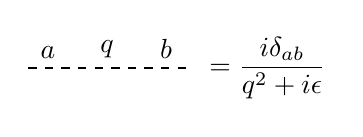
\begin{tikzpicture}
              \draw[dashed](-1,0)node[above, midway]{$\momright{q}$}--
              node[very near start,above]{$a$}
              node[very near end,above]{$b$}
              (1,0)
              node[right=5]{$\displaystyle=\frac{i\delta_{ab}}{q^2+i\epsilon}$};
          \end{tikzpicture}
          \\
          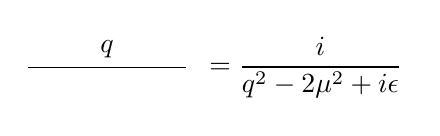
\begin{tikzpicture}
              \draw(-1,0)node[above, midway]{$\momright{q}$}--(1,0)
              node[right=5]{$\displaystyle=\frac{i}{q^2-2\mu^2+i\epsilon}$};
          \end{tikzpicture}
          \\
          %vertex 3 sigma
          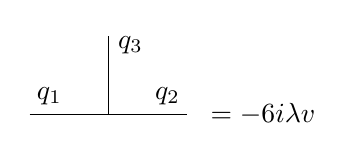
\begin{tikzpicture}
              \draw(-1,0)--node[above, near start]{$\momright{q_1}$}(0,0);
              \draw(0,0)--node[above, near end]{$\momleft{q_2}$}(1,0)node[right=5]{$\displaystyle=-6i\lambda v$};
              \draw(0,0)--node[right,very near end]{$\momdownu{q_3}$}(0,1);
              \vertexb{0,0};
          \end{tikzpicture}
          \\
          %vertex 2 pion 1 sigma
          \begin{tikzpicture}
              \draw[pion](-1,0)--node[above, near start]{$\momright{q_1},a$}(0,0);
              \draw[pion](0,0)--node[above, near end]{$\momleft{q_2},b$}(1,0)node[right=5]{$\displaystyle=-2i\lambda v\, \delta_{ab}$};
              \draw(0,0)--node[right, very near end]{$\momdownu{q_3}$}(0,1);
              \vertexb{0,0};
          \end{tikzpicture}
          \\
          %vertex 2 pion 2 sigma
          \begin{tikzpicture}
              \draw[pion](225:1)--node[above, near start,sloped]{$\momright{q_1},a$}(0,0);
              \draw[pion](135:1)--node[above, near start,sloped]{$\momright{q_2},b$}(0,0);
              \draw(-45:1)--node[below, near start,sloped]{$\momleftu{q_3}$}(0,0);
              \draw(45:1)-- node[below, near start,sloped]{$\momleftu{q_4}$}(0,0);
              \vertexb{0,0};
              \node[right=25] at (0,0){$\displaystyle=-2i\lambda\, \delta_{ab}$};
          \end{tikzpicture}
          \\
          %vertex 4 sigma
          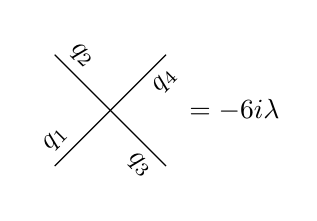
\begin{tikzpicture}
              \draw(225:1)--node[above, near start,sloped]{$\momright{q_1}$}(0,0);
              \draw(135:1)--node[above, near start,sloped]{$\momright{q_2}$}(0,0);
              \draw(-45:1)--node[below, near start,sloped]{$\momleftu{q_3}$}(0,0);
              \draw(45:1)-- node[below, near start,sloped]{$\momleftu{q_4}$}(0,0);
              \vertexb{0,0};
              \node[right=25] at (0,0){$\displaystyle=-6i\lambda$};
          \end{tikzpicture}
          \\
          %vertex 4 pion
          \begin{tikzpicture}
              \draw[pion](225:1)--node[above, near start,sloped]{$\momright{q_1},a$}(0,0);
              \draw[pion](135:1)--node[above, near start,sloped]{$\momright{q_2},b$}(0,0);
              \draw[pion](-45:1)--node[below, near start,sloped]{$\momleftu{q_3},c$}(0,0);
              \draw[pion](45:1)-- node[below, near start,sloped]{$\momleftu{q_4},d$}(0,0);
              \vertexb{0,0};
              \node[right=25] at (0,0){$\displaystyle=-2i\lambda \left(\delta_{ab}\delta_{cd}+\delta_{ac}\delta_{bd}+\delta_{ad}\delta_{bc}\right)$};
          \end{tikzpicture}


    \item[(c)] Show that the pion fields remain massless when the one-loop corrections are included.~Remember that the physical particle mass is obtained from the self-energy, in particular, for a pion with external momentum $p$ as
          \begin{equation}
              m_{\pi}^2=\Sigma_{\pi}(p^2=m_{\pi}^2)\,.
              \label{eq:mPi}
          \end{equation}
          The leading diagrams contributing to $\Sigma_{\pi}$ are shown in Fig.~\ref{fig:SigmaPi}, where a dashed line denotes the pion field and a solid line denotes the sigma field. Write down their mathematical expressions and show that Eq.~\eqref{eq:mPi} holds true for $m_{\pi}^2=0$.

          \begin{figure}[h]
              % tadpole sigma above	
              \begin{subfigure}{0.17 \textwidth}
                  \centering
                  \begin{tikzpicture}
                      \draw[white, very thin](-1,0)--(-1,2);
                      \draw[pion](-1,0)--(1,0);
                      \draw(0,0)--(0,1);
                      \draw (0,1) arc[start angle=-90, end angle=270, radius=0.5cm];
                      \vertexb{0,0}; \vertexb{0,1};
                  \end{tikzpicture}
                  \caption{}
              \end{subfigure}
              % tadpole sigma		
              \begin{subfigure}{0.17 \textwidth}
                  \centering
                  \begin{tikzpicture}
                      \draw[white, very thin](-1,0)--(-1,2);
                      \draw[pion](-1,0)--(1,0);
                      \draw (0,0) arc[start angle=-90, end angle=270, radius=0.5cm];
                      \vertexb{0,0};
                  \end{tikzpicture}
                  \caption{}
              \end{subfigure}
              % tadpole pion	above		
              \begin{subfigure}{0.17 \textwidth}
                  \centering
                  \begin{tikzpicture}
                      \draw[white, very thin](-1,0)--(-1,2);
                      \draw[pion](-1,0)--(1,0);
                      \draw(0,0)--(0,1);
                      \draw[pion] (0,1) arc[start angle=-90, end angle=270, radius=0.5cm];
                      \vertexb{0,0}; \vertexb{0,1};
                  \end{tikzpicture}
                  \caption{}
              \end{subfigure}
              % tadpole pion		
              \begin{subfigure}{0.17 \textwidth}
                  \centering
                  \begin{tikzpicture}
                      \draw[white, very thin](-1,0)--(-1,2);
                      \draw[pion](-1,0)--(1,0);
                      \draw[pion] (0,0) arc[start angle=-90, end angle=270, radius=0.5cm];
                      \vertexb{0,0};
                  \end{tikzpicture}
                  \caption{}
              \end{subfigure}
              % sunset	
              \begin{subfigure}{0.27 \textwidth}
                  \centering
                  \begin{tikzpicture}
                      \draw[white, very thin](-2,0)--(-2,2);
                      \draw[pion](-2,0)--(2,0);
                      \draw (1,0) arc[start angle=0, end angle=180, radius=1];
                      \vertexb{1,0}; \vertexb{-1,0};
                  \end{tikzpicture}
                  \caption{}
              \end{subfigure}
              \caption{The leading order diagrams contributing to $\Sigma_{\pi}$.}
              \label{fig:SigmaPi}
          \end{figure}
          \emph{Hint 1:} The last diagram has a symmetry factor 1, all others have a symmetry factor 2. The mathematical expression of each diagram has to be divided by its symmetry factor.

          \emph{Hint 2:} How to treat the pion indices of pion loops?


          \emph{Hint 3:} You can write the result of any diagram $n$ as $\Sigma_n = \delta_{i j} X^n \times I_n$, where $X^n$ is some coefficient that contains the symmetry factor of diagram $n$ and $I_n$ contains only the one-loop part.~Make sure that when the loop contains one propagator, then $I_n$ can be either $ I_n  = I^1 = \int \frac{d^d l }{(2\pi)^d } \frac{i}{l^2 - 2 \mu^2 + i \epsilon }$ or $I_n = I^2  = \int \frac{d^d l }{(2\pi)^d} \frac{i}{l^2  + i \epsilon }$ and  for two propagators in the loop we have $I_n = I^3 = \int \frac{d^d l }{(2\pi)^d } \frac{i}{(l-p)^2 + i \epsilon } \frac{i}{l^2 - 2 \mu^2 + i \epsilon}$, where because of $m_\pi^2 = 0$ we have $p^2 = 0$.

          \emph{Hint 4:} You can keep the loop integrals without carrying out the momentum integration.~But you should express $I^3$ in terms of $I^1$ and $I^2$.~For that, you can use Feynman parametrization to show the independence of the angular part as follows:

          \begin{eqnarray}
              \int d^d l\,\frac{1}{(l-p)^2\left(l^2-2\mu^2\right)}|_{p^2=0}
              \!\!\!&=&\!\!\!
              \int d x\, \int \dd^d l\, \left[x(p-l)^2+(1-x)(l^2-2\mu^2)\right]|_{p^2=0}
              \nonumber
              \\
              \!\!\!&=&\!\!\!
              \int d x\, \int \dd^d l\, \left[(l-px)^2-p^2x^2+xp^2+(1-x)2\mu^2\right]\big\vert_{p^2=0}
              \nonumber
              \\
              \!\!\!&\overset{l-px\rightarrow l}{=}&\!\!\!
              \int \dd x\, \int \dd^d l\, \left[l^2-p^2x^2+xp^2+(1-x)2\mu^2\right]|_{p^2=0}
              \nonumber
              \\
              \!\!\!&=&\!\!\!
              \int d x\, \int \dd^d l\, \left[xl^2+(1-x)(l^2-2\mu^2)\right]=\int d^d l\,\frac{1}{l^2\left(l^2-2\mu^2\right)}
              \,,
              \nonumber
              \\
          \end{eqnarray}

          Use your results and make partial fraction decomposition to write the self-energy as $\Sigma_{a}+\Sigma_{b}+\Sigma_{c}+\Sigma_{d}+\Sigma_{e} = \lambda \delta_{i j} \left(  \alpha I^1 + \beta I^2 \right)$, and show that $\alpha = \beta = 0$.
\end{itemize}
\emph{Remark:} That pions are massless even beyond the classical (tree level) calculation is a non-trivial feature and is due to the SSB, which ``protects'' the (zero) pion mass.

\begin{itemize}
    \item[(d)] Compute the scattering amplitude for
          $\pi_i(p_1) \pi_j(p_2) \rightarrow \pi_k(p_3) \pi_l(p_4)$
          at tree level.
          %to leading order in $\lambda$. 
          Show that these diagrams sum up to zero at the threshold $\vec{p}_i=\vec{0}$.
\end{itemize}
\emph{Remark:} It is a general feature that the interactions of Goldstone bosons vanish for low energies.~This is the foundation for the construction of \emph{Chiral Perturbation Theory}, where all pion interaction terms are either suppressed by insertions of the quark masses (explicit chiral symmetry breaking terms) or have to contain derivatives.

\subsection{Compensator field for chiral transformations}
\noindent
The pion fields $(\pi^0, \pi^+, \pi^-)$ are conveniently expressed in the chiral effective Lagrangian in terms of their cartesian components $\pi^a \in \{ \pi^1, \pi^2, \pi^3\}$ as follows:
\begin{eqnarray}
    \pi^0
    =
    \pi^3
    ,\,
    \pi^+
    =
    \frac{1}{\sqrt{2}} \left( \pi^1 - i  \pi^2 \right)
    ,\,
    \pi^-
    =
    \frac{1}{\sqrt{2}} \left( \pi^1 + i  \pi^2 \right)
    \,.
    %\pi^1& =& \frac{1}{\sqrt{2}} \left( \pi^+ + \pi^- \right),\, \pi^2 = \frac{i}{\sqrt{2}} \left( \pi^+ -\pi^- \right),\, \pi^3 =  \pi^0.
    \label{PhyIso}
\end{eqnarray}
In the two-flavor sector, the pion fields $\pi^a$ appear in the Lagrangian via the matrix $U = u^2$, which can be parametrized as follows:
\begin{eqnarray}
    U
    &=&
    \mathbf{1}_{2\times 2} + i \frac{\boldsymbol{\tau}\,{\cdot}\,\boldsymbol{\pi}}{F} - \frac{\boldsymbol{\pi}^2}{2 F^2} -  i \alpha \frac{\boldsymbol{\pi}^2 \, \boldsymbol{\tau}{\cdot}{\boldsymbol{\pi}}}{F^3} + (8 \alpha -1)\frac{\boldsymbol{\pi}^4}{8 F^2} + \mathcal{O}(\boldsymbol{\pi}^5)    % 
    \label{a1244}
    \,,
\end{eqnarray}
where $\alpha$ is an arbitrary constant which reflects the freedom in parametrizing the matrix $U$, $\tau^a$ are the Pauli matrices and $F$ is the pion decay constant in the chiral limit.~

The pionic matrix $U$ transforms under  chiral rotations as follows:
\begin{eqnarray}
    U
    \mapsto  L U R^\dagger
    \,,
\end{eqnarray}
where $R$ and $L$ are spacetime-independent $SU(2)$ matrices.~From the above equation, it follows that the matrix $u$ transforms under global chiral rotations as follows:
\begin{eqnarray}
    u
    \mapsto  u^\prime = \sqrt{L u R^\dagger} \equiv L u h^{-1} = h u R^\dagger
    \,,
\end{eqnarray}
where the spacetime-dependent unitary matrix $h = h(L, R, U) = \sqrt{L U R^\dagger}^{-1} L \sqrt{U}$ is sometimes referred to as a compensator field.

Calculate the explicit form of the compensator field $h$ for infinitesimal chiral transformations using Eq.~(\ref{a1244}) and keeping only terms that are at most linear in the pion fields.~Verify also that $h$ indeed reduces to the isospin transformation for $L = R = V$.





\subsection{Fermionic charges of isospin symmetry}
\noindent
We consider the isospin symmetry of nucleons, which is approximately realized in nature since proton and neutron have almost the same mass $m_N$.
As for spin, the symmetry group is SU(2) with the Lie algebra su(2), which has the Levi-Civita symbol $\varepsilon_{abc}$ as structure constants and the isospin Pauli matrices
\begin{equation}
    \tau_1 = \begin{pmatrix} 0&1\\ 1&0 \end{pmatrix}, \qquad
    \tau_2 = \begin{pmatrix} 0&-i\\ i&0 \end{pmatrix}, \qquad
    \tau_3 = \begin{pmatrix} 1&0\\ 0&-1 \end{pmatrix}, \qquad
    \text{with } \vec{\tau} := (\tau_1, \tau_2, \tau_3)
\end{equation}
divided by 2 as basis (or generators) of the fundamental representation, i.e., they fulfill the equation
\begin{equation}
    \left[ \frac{\tau_i}{2}, \frac{\tau_j}{2} \right] = i \varepsilon_{ijk} \frac{\tau_k}{2} .
\end{equation}
Consider the free fermion Lagrangian
\begin{equation}
    \mathcal{L} = \bar\Psi ( i \slashed{\partial} - m_N ) \Psi ,
\end{equation}
where the two-component field vector $\Psi := (p,n)^T$ is build of the proton field $p$ and neutron field $n$ which themselves are Dirac spinors, such that $\Psi$ has two indices. It transforms under isospin via the fundamental representation as follows:
\begin{equation}
    \label{eq:transformation_isospin}
    \Psi(x) \rightarrow \Psi'(x) = \Psi(x) + i \epsilon_i \frac{\tau_i}{2} \Psi(x) = \Psi(x) + i \vec\epsilon \cdot \frac{\vec\tau}{2} \Psi(x) .
\end{equation}
The (components of the) fermion field operators $\Psi$ must obey the anticommutation relations
\begin{equation}
    \label{eq:equ-time_commutation_fermions}
    \{\Psi_{r,\alpha}(t,\vec x), \Psi_{s,\beta}^\dagger(t,\vec y)\} = \delta^3(\vec x - \vec y) \delta_{rs} \delta_{\alpha\beta} , \qquad
    \{\Psi_{r,\alpha}(t,\vec x), \Psi_{s,\beta}(t,\vec y)\} = 0 = \{\Psi_{r,\alpha}^\dagger(t,\vec x), \Psi_{s,\beta}^\dagger(t,\vec y)\} ,
\end{equation}
where $r,s \in \{1,2\}$ denote isospin indices and $\alpha,\beta \in \{1,2,3,4\}$ denote Dirac indices.~We want to show that the su(2) charge operators\footnote{Appendix \ref{B:Apendix} contains a discussion that shows how to obtain the charges.} w.r.t.\ $\mathcal{L}$ form a Hilbert space representation of the Lie algebra, i.e.,
\begin{equation}
    \label{eq:lie_algebra}
    [Q_i(t), Q_j(t)] = i \varepsilon_{ijk} Q_k(t) .
\end{equation}
We want to explicitly prove this in the following.

\begin{itemize}
    \item[(a)]
          Find the three charges as
          \begin{equation}
              \vec{Q}(t) = \int \dd^3 x \: \Psi^\dagger(t, \vec x) \frac{\vec\tau}{2} \Psi(t, \vec x) .
          \end{equation}

    \item[(b)]
          Show Eq.~\eqref{eq:lie_algebra}.

          \textit{Hint:} First verify $[AB,CD] = A \{B,C\} D - A C \{B,D\} + \{A,C\} D B - C \{A,D\} B$. Note that to apply this, the fields $\Psi, \bar\Psi$ must be written in components.
\end{itemize}



\subsection{Effective Lagrangian and heavy-baryon reduction of the free Dirac Lagrangian}
\noindent
\begin{itemize}
    \item[(a)] A quantum field theory for two scalar fields interacting with a Yukawa-like coupling, as considered in the lecture, is given by the Lagrangian
          \begin{gather}
              \L=
              \frac{1}{2}\partial_{\mu}\phi\partial^{\mu}\phi
              -\frac{1}{2}m^2\phi^2
              +\frac{1}{2}\partial_{\mu}\Phi\partial^{\mu}\Phi
              -\frac{1}{2}M^2\Phi^2
              -\frac{\lambda}{2}\phi^2\Phi.
              \label{eq:Leff}
          \end{gather}
          Assuming that $\phi$ and $\Phi$ correspond to a light and a heavy particle with masses $m\ll M$, one can derive an effective Lagrangian that involves only the light degrees of freedom. For processes on tree diagram level (i.e. on the classical level), this can be easily done by using the equation of motion (EOM).

          Derive the EOM for the heavy field and show that it is formally solved by
          \begin{gather}
              \Phi=\frac{\lambda}{2}\frac{1}{-\Box -M^2}\phi^2,
              \label{eq:formal_sol}
          \end{gather}
          where we use the D'Alembert operator $\Box=\partial_{\mu}\partial^{\mu}$.
          %\footnote{You don't have to properly solve the EOM, but instead give a formal solution that includes seemingly mathematically not well-defined operators.}
          Plug this solution back into the full Lagrangian and show that the Lagrangian can be written as follows\footnote{You should transform and simplify the effective Lagrangian such that it is only expressed in multiples of $\phi$, $(\partial_{\mu}\phi)$ and $(\partial^{\mu}\phi)$
              (and is especially free from expressions like $\partial_{\mu}(\phi^2)$ or $\partial_{\mu}\partial^{\mu}\phi$).}
          \begin{align}
              \L & =\L_0^{\phi}+\frac{\lambda^2}{8}\frac{1}{M^2}\phi^2 \frac{1}{1+\frac{\Box}{M^2}}\phi^2
              \,.
          \end{align}
          Use the formal Taylor expansion in $\frac{\Box}{M^2}$ to show that the effective Lagrangian up to and including order $(1/M)^4$ can be written as\footnote{Note that you can do integration by parts in the Lagrangian, without changing physics, because there appears an integral in the action $S=\int\dd^ 4 x \L$ and the field are expected to vanish for large $x$.}
          \begin{gather}
              \L_{\text{eff}}=
              \frac{1}{2}\partial_{\mu}\phi\partial^{\mu}\phi
              -\frac{1}{2}m^2\phi^2
              +\frac{\lambda^2}{8}\frac{1}{M^2}\phi^4
              -\frac{\lambda^2}{8}\frac{1}{M^4}\phi^2 \Box \phi^2
              %+\O\left(\left(\frac{m^2}{M^2}\right)^3\right).
              +\O\left(\frac{1}{M^6}\right).
          \end{gather}

    \item[(b)]As next, consider the free Dirac Lagrangian given by

          \begin{eqnarray}
              \mathcal{L} = \bar \Psi \left( i \slashed{\partial}  - m \right) \Psi
              \,.
          \end{eqnarray}
          The nucleon mass is not expected to vanish in the chiral limit and it is not small compared to the chiral symmetry-breaking scale, thus complicating the expansion in powers of momenta by breaking the power counting of chiral perturbation theory.~One way to solve this problem is the construction of heavy-baryon chiral perturbation theory (HBChPT), where the starting idea is to separate the nucleon four-momenta $p$ into a large part close to the on-shell kinematics and a soft part $k_p$, as
          \begin{gather}
              p^{\mu}=m v^{\mu} + k_p^{\mu},\quad \text{where}\quad v\cdot v=1, v^0\geq 1\,.
          \end{gather}

          %\comment{NC: Better take the task with Bilinears? This would need more informations to $N$, $H$ and $\vs N$ and $\slashed{v}H$}

          The relativistic nucleon field is then decomposed into a large and a small component
          \begin{align}
              \Psi   & =e^{-im\,v\cdot x}\left[N_v(x)+H_v(x)\right],
              \\
              N_v(x) & =e^{im\,v\cdot x} P_{v+}\Psi,
              \\
              H_v(x) & =e^{im\,v\cdot x} P_{v-}\Psi,
          \end{align}
          using the projection operators
          \begin{equation}
              P_{v\pm}=\frac{\eins\pm\vs}{2}
              \,.
          \end{equation}
          You can convince yourself that they fulfill
          \begin{equation}
              P_{v+}+P_{v-}=\eins\,,\quad
              P_{v\pm}^2=P_{v\pm}\,,\quad
              P_{v\pm}P_{v\mp}=0\,.
          \end{equation}
          Show that the free Dirac Lagrangian can be rewritten as follows:

          \begin{eqnarray}
              \mathcal{L}
              &=&
              \bar N_v(x) \left( i v {\cdot} \partial \right) N_v(x) -  \bar H_v(x) \left( i v {\cdot} \partial + 2m  \right) H_v(x) +  \bar N_v(x) \left( i \slashed{\partial}_\perp \right) H_v(x)
              \nonumber
              \\
              &+& \bar H_v(x) \left(  i \slashed{\partial}_\perp  \right) N_v(x)\,,
              \label{DLag}
          \end{eqnarray}
          where $\partial_\perp \equiv \partial -  (v {\cdot} \partial) v$\,.
\end{itemize}
Proceed now similarly to the case of scalar fields in (a) and derive the EOM for the field $\bar H_v(x)$ and plug the solution back into the full Lagrangian in Eq.~\eqref{DLag} and expand in powers of
$1/m$ to derive the effective Lagrangian up to and including the next-to-leading order in $1/m$.


\subsection*{Appendix: Functional derivatives}
\label{A:1}
Functions take elements of an arbitrary set and map it to exactly one element of another set, e.g., $f\colon \mathbb{R}^n \rightarrow \mathbb{R}^m$.
Functionals take elements from function spaces, such as $L^2(\mathbb{R}^n)$ or $C^n(\mathbb{R}^m)$, and map them to the complex or real numbers.
Two examples are the integral with the Dirac delta function or the norm on $L^2(\mathbb{R}^n)$;
in this case we have $F\colon L^2(\mathbb{R}^n)\to \mathbb{R}$.

In physics the most common example is the action functional $S[x]$.
Closely connected to the action is the \emph{variational principle}, which derives the equation of motion from the action.
To explain this, consider a functional $F[\phi]$ and assume that an arbitrary small variation $\phi(x) \to \phi(x) + \epsilon h(x)$ is performed.
Mathematically, this describes the rate of change of $F[\phi]$ when $\phi$ is perturbed at the point $x$ and is calculated by taking the \emph{functional derivative}.

The functional derivative is defined similarly to the ordinary derivative:
\begin{align}
    \int d^4 z\, \frac{\delta F[\phi]}{\delta \phi(z)} h(z)
    =
    \lim \limits_{\varepsilon \rightarrow 0}\frac{F[\phi+\varepsilon h]-F[\phi]}{\varepsilon}\,,
\end{align}
where $h$ is an arbitrary test function and the limit $\varepsilon \to 0 $ is to be taken before any integration.

Note that the definition above corresponds to the directional derivative, here in the direction of $h$ and by using the Dirac delta function
$h(z)=\delta(z-x)$
the left hand side of the equation simplifies to
$\frac{\delta F[\phi]}{\delta \phi(x)}$.

Using the definition it can be shown, similar to the proofs in for the classical derivative, that the functional derivative is linear and follows the product rule:
\begin{align}
    \frac{\delta(\alpha F+\beta G)[\phi]}{\delta \phi(x)}
    ={} &
    \alpha \frac{\delta F[x]}{\delta \phi(x)}+\beta \frac{\delta G[\phi]}{\delta \phi(x)}\,,
    \\
    \frac{\delta( F G)[\phi]}{\delta \phi(x)}
    ={} &
    \frac{\delta F[\phi]}{\delta \phi(x)}G[\phi]+ F[\phi]\frac{\delta G[\phi]}{\delta \phi(x)}\,.
\end{align}
Because the functional derivative fulfills these two properties, it is also a derivative in the strict mathematical sense.
Many other properties of functional derivatives are the same as for ordinary derivatives, like the chain rule.

Several simple examples of functional derivatives are given in the following list:
\begin{itemize}
    \item[(a)] $\frac{\delta \phi(x)}{\delta \phi(y)} =  \delta^4(x-y)$
    \item[(b)] $\frac{\delta}{\delta \phi(y)} \int d^4 x\, \phi(x) g(x) = g(y)$
    \item[(c)] $\frac{\delta}{\delta \phi(y)} \int d^4 x\, (\phi(x))^n = n (\phi(y))^{n-1}$
    \item[(d)] $\frac{\delta}{\delta\phi\left(z\right)}\exp\left(\int d^4 x\,\phi\left(x\right)J\left(x\right)\right) = J(z) \exp\left(\int d^4 x\,\phi\left(x\right)J\left(x\right)\right)$

          (The exponential function is understood as its corresponding power series here.)
\end{itemize}

\subsection*{Appendix: Noether's theorem}
\label{B:Apendix}
\textbf{Definition:} Given a set of fields $\phi_i$ (to be understood as scalar fields or components of vector fields), an infinitesimal global transformation
\begin{equation}
    \label{transformation}
    \begin{split}
                       & x^\mu \rightarrow x'^\mu = f^\mu(x, \epsilon) = x^\mu + \epsilon^a A^\mu_a (x) , \qquad \phi_i (x) \rightarrow \phi'_i (x') = \phi_i (x) + \epsilon^a F_{i,a} (\phi(x)) \\
        \Rightarrow \; & \phi'_i (x) = \phi_i (x) + \underbrace{\left( F_{i,a} (\phi(x)) - A^\mu_a (x) \partial_\mu \phi_i (x) \right)}_{\displaystyle =: \Delta_{i,a}} \epsilon^a
        \equiv \phi_i (x) + \delta \phi_i (x),
    \end{split}
\end{equation}
with the parameters $\epsilon^a$ ($a = 1, \dots, N)$ is called a \textit{symmetry} if it leaves invariant the action
\begin{equation}
    \label{eq:action_invariance}
    S = \int_{\Omega} \dd^4 x \: \mathcal{L}(\phi(x), \partial_\mu \phi(x)) , \qquad \text{i.e.,} \quad
    S = S'
    = \int_{\Omega' = f(\Omega, \epsilon)} \dd^4 x' \: \mathcal{L}(\phi'(x'), \partial' \phi'(x')).
\end{equation}

\textbf{Theorem:} For each symmetry with corresponding transformation \eqref{transformation} and $\phi_i$ satisfying the classical equations of motion (EOMs)
\begin{align}
    \frac{\partial \mathcal{L}}{\partial \phi_i} - \partial_\mu \frac{\partial \mathcal{L}}{\partial(\partial_\mu \phi_i)} = 0,
\end{align}
there exist $N$ conserved \textit{Noether currents}
\begin{equation}
    \label{eq:noether_current}
    j^\mu_a = -\frac{\partial \mathcal{L}}{\partial (\partial_\mu \phi_i)} \Delta_{i,a} - A^\mu_a \mathcal{L} \qquad \text{which fulfill} \qquad \partial_\mu j^\mu_a (x) = 0 .
\end{equation}
As a direct implication, one obtains the conserved \textit{Noether charges}
\begin{equation}
    Q_a = \int_{\mathbb{R}^3} \dd^3 x \: j^0_a (x) \qquad \text{with} \qquad \frac{\dd}{\dd t} Q_a = 0 .
\end{equation}

\subsection*{Appendix: Method of Gell-Mann and L\'evy}
%from QFT 1 SS 21, H5.1
%and Scherer, Schindler, A Primer for Chiral Perturbation Theory, pp. 13 f.
%similarities to THP SS 17, H2.3

The above definition is written for a \textit{global} symmetry where the transformation parameters $\epsilon^a$ are constant.
For calculating a Noether current, it may however be useful to promote this global symmetry to a \textit{local} symmetry, i.e., to assume that $\epsilon^a$ are functions of space-time: $\epsilon^a \rightarrow \epsilon^a(x)$.
Using the EOMs, one can show that the current and its divergence are then obtainable from
\begin{align}
    \label{eq:gell-mann_levy}
    j^\mu_a = -\frac{\partial(\Delta \mathcal{L})}{\partial(\partial_\mu \epsilon_a)}
    \qquad \text{and} \qquad
    \partial_\mu j^\mu_a = -\frac{\partial(\Delta \mathcal{L})}{\partial \epsilon_a} ,
\end{align}
with the action difference $\int_\Omega \dd^4 x \: \Delta \mathcal{L} = \int_{\Omega'} \dd^4 x' \: \mathcal{L}(\phi'(x'), \partial' \phi'(x')) - \int_\Omega \dd^4 x \: \mathcal{L}(\phi(x), \partial \phi(x))$ given by
\begin{align}
    \int_\Omega \dd^4 x \: \Delta \mathcal{L} = \int_\Omega \dd^4 x \: \left( \partial_\mu( \epsilon^a(x) A^\mu_a(x) \mathcal{L}(\phi(x), \partial \phi(x)) )
    + \frac{\partial \mathcal{L}}{\partial \phi_i} \delta \phi_i(x)
    + \frac{\partial \mathcal{L}}{\partial(\partial_\mu \phi_i)} \delta(\partial_\mu \phi_i(x)) \right)
    \quad \forall \; \Omega.
\end{align}

Requiring the stronger symmetry constraint $\Omega' = \Omega$, the symmetry condition $S=S'$ of Eq.~\eqref{eq:action_invariance} becomes
$\dd^4 x \mathcal{L}(\phi(x), \partial \phi(x)) = \dd^4 x' \mathcal{L}(\phi'(x'), \partial' \phi'(x'))$. If further $\dd^4 x = \dd^4 x'$, the symmetry condition is equivalent to the invariance of the Lagrangian: $\mathcal{L}(\phi(x), \partial \phi(x)) = \mathcal{L}(\phi'(x'), \partial' \phi'(x'))$.

In particular, this is fulfilled if the coordinates themselves are invariant, i.e., $x^\mu \rightarrow x^\mu$ or $A_a^\mu = 0$.
In this case, the Noether current \eqref{eq:noether_current} simplifies to $j^\mu_a = -\frac{\partial \mathcal{L}}{\partial (\partial_\mu \phi_i)} F_{i,a}$ and $\Delta \mathcal{L}$ reduces to the Lagrangian variation
\begin{align}
    \delta \mathcal{L} = \frac{\partial \mathcal{L}}{\partial \phi_i} \delta \phi_i + \frac{\partial \mathcal{L}}{\partial(\partial_\mu \phi_i)} \partial_\mu \delta \phi_i,
    \qquad \text{so that Eq.~\eqref{eq:gell-mann_levy} becomes} \quad
    j^\mu_a = -\frac{\partial(\delta \mathcal{L})}{\partial(\partial_\mu \epsilon_a)},\quad
    \partial_\mu j^\mu_a = -\frac{\partial(\delta \mathcal{L})}{\partial \epsilon_a} ,
\end{align}
which in this form can be a very convenient tool, because $\delta \mathcal{L}$ can be easily computed for a given transformation. Moreover, the method also works for ``non-conserved currents'' $\partial_\mu j^\mu_a \neq 0 \neq \delta \mathcal{L}$, i.e., if the transformation is not a symmetry.

\end{document}
